\documentclass[10pt]{beamer}
\usepackage{amsmath}
\usepackage{amssymb}
\usepackage{geometry}
\usepackage{graphicx}
\usepackage{url}

\begin{document}

\begin{frame}
\large Lecture 13: Chi-Square Tests\\
STAT 630, Fall 2021
\end{frame}

\begin{frame}{The $\chi^2$ Distribution}
\begin{itemize}
\item Let $Z \sim N(0,1)$, then $Z^2$ follows a chi-square distribution with 1 degree of freedom, denoted by $Z^2 \sim \chi^2_1$.
\vspace{10pt}
\item Let $Z_1, Z_2, \cdots, Z_n$ be independent random variables each following $N(0,1)$.  Let $V = \sum_{i=1}^n Z_i^2$.  Then $V$ follows a chi-square distribution with $n$ degrees of freedom, denoted by $V\sim \chi^2_n$.  
\vspace{10pt}
\item Let $V \sim \chi^2_n$, then $E(V) = n$ and $Var(V) = 2n$.  
\end{itemize}
\end{frame}

\begin{frame}
Plot of $\chi^2_n$ distribution with different degrees of freedom $n$:
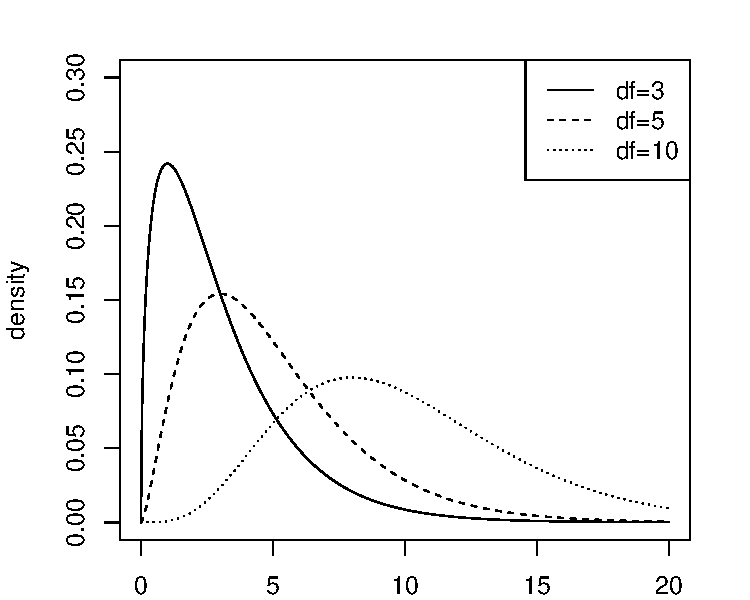
\includegraphics[scale=0.6]{chi.pdf}
\end{frame}

\begin{frame}
\textbf{Example}: Let $Z_1, Z_2, \cdots, Z_{10}$ be independent random variables from $N(0,1)$.  Let $V = \sum_{i=1}^{10} Z_i^2$.
\smallskip

\begin{enumerate}[(a)]
\item What distribution does $V$ follow?  What is $E(V)$ and $Var(V)$?\\
\vspace{2.5cm}
% \emph{Solution}: $V$ follows a chi-square distribution with 10 degrees of freedom; or we can write $V \sim \chi^2_{10}$.  $E(V) = 10$ and $Var(V) = 2\cdot 10 = 20$.
\item Calculate $P(V > 15)$\\
\vspace{2.5cm}
% \emph{Solution}: $P(V > 15) = 1 - P(V < 15) = 1 - \texttt{pchisq(15, df=10)} = \Sexpr{round(1-pchisq(15, df=10), 3)}$
\end{enumerate}
\end{frame}



% \begin{frame}
% \large
% \textbf{Chi-Square Test of Independence}
% \end{frame}

%------------------------------------
\begin{frame}{Chi-Square Test of Independence}
A \textbf{chi-square test of independence} is used to evaluate whether or not two categorical variables, expressed as a contingency table, are independent of each other.\\
\vspace{10pt}

\textbf{Example}:  The General Social Survey (GSS) surveyed a random sample of Americans in 2002.  As part of this survey each participant was asked whether they favor or oppose the death penatly.  The suvey also collected data on the education level of each participant.  Does the survey provide evidence of a relationship between education level and postion on the death penalty?\\
\vspace{10pt}

$H_0$: Education and position on death penalty are independent\\
$H_A$: Education and position on death penalty are not independent
\end{frame}


%------------------------------------
\begin{frame}

Contingency table of the data (table of observed counts):\\
\vspace{5pt}

\begin{table}[ht]
\centering
\begin{tabular}{rrrr}
\hline
\multicolumn{1}{c}{} &
\multicolumn{2}{c}{Death Penalty?} &
\multicolumn{1}{c}{}\\
\cline{2-3}
 & Favor & Oppose & Row Total \\
\hline
Left HS & 117 & 72 & 189 \\
HS & 511 & 200 & 711 \\
Jr Col & 71 & 16 & 87 \\
Bachelors & 135 & 71 & 206 \\
Graduate & 64 & 50 & 114 \\
\hline
Column Total & 898 & 409 & 1307 \\
\hline
\end{tabular}
\end{table}

\end{frame}


%------------------------------------
\begin{frame}
Assuming that the null hypothesis is true, and the two categorical variables are independent, we can construct a table of the \textbf{expected counts}.
\begin{itemize}
\item $n$: overall total number of observations\\
\item $R_i$: total for row $i$\\
\item $C_j$: total for column $j$\\
\end{itemize}
\vspace{10pt}

Then the expected count in row $i$ and column $j$ is given by
\begin{align*}
E_{ij} = \frac{R_i \cdot C_j}{n}
\end{align*}

% \small
% \textbf{Remark}:  This follows from probabilty since two events $A$ and $B$ are independent if $P(A \text{ and } B) = P(A)P(B)$.  For example, if we assume independence, $P(\text{HS and Oppose}) = P(\text{HS})P(\text{Oppose}) = \frac{711}{1307} \cdot \frac{409}{1307}$, and so the expected number of HS graduates that oppose the death penatly is $1307 \cdot \frac{711}{1307} \cdot \frac{409}{1307} = \frac{711 \cdot 409}{1307} = 222.5$.  
%Also going, back to the example, $898/1307=68.7$\% of participants favored the death penalty and $409/1307=31.3$\% opposed. Since there are 711 HS graduates, for example, if we assume independence, then we would expect $(0.687)(711)=488.5$ of HS gradutes to favor and $(0.313)(711)=222.5$ to oppose the death penalty.    
\end{frame}

\begin{frame}
\vspace{-4cm}
Notes:
\end{frame}

%------------------------------------
\begin{frame}
\vspace{-1cm}
Table of expected counts:

\begin{table}[ht]
\centering
\begin{tabular}{rrrr}
\hline
\multicolumn{1}{c}{} &
\multicolumn{2}{c}{Death Penalty?} &
\multicolumn{1}{c}{}\\
\cline{2-3}
& Favor & Oppose & Row Total \\ 
\hline
Left HS & 129.9 & 59.1 & 189\\ 
HS & 488.5 & 222.5 & 711\\ 
Jr Col & 59.8 & 27.2 & 87\\ 
Bachelors & 141.5 & 64.5 & 206\\ 
Graduate & 78.3 & 35.7 & 114\\ 
\hline
Column Total & 898 & 409 & 1307\\ 
\hline
\end{tabular}
\end{table}
%\vspace{10pt}

% For example, for the HS graduates,\\ 
% $E_{21} = R_2 \cdot C_1 / n = 711 \cdot 898 / 1307 = 488.5$\\  
% $E_{22} = R_2 \cdot C_2 / n = 711 \cdot 409 / 1307 = 222.5$

\end{frame}

%------------------------------------
\begin{frame}
Chi-square test statistic:
\begin{align*}
\chi^2 &= \sum_{\text{all cells}} \frac{(\text{Observed} - \text{Expected})^2}{\text{Expected}}\\
&= \sum_{i=1}^I \sum_{j=1}^J \frac{(O_{ij} - E_{ij})^2}{E_{ij}},
\end{align*}
where $O_{ij}$ is the observed count, $I$ is the number of rows, and $J$ is the number of columns.\\
\vspace{10pt}
The degrees of freedom is $(I-1)(J-1)$.\\
\end{frame}

%------------------------------------
\begin{frame}
For the example, the value of test statistic is\\
\begin{align*}
\chi^2 &= \frac{(117-129.9)^2}{129.9} + \frac{(72-59.1)^2}{59.1} + \frac{(511-488.5)^2}{488.5} + \frac{(200-222.5)^2}{222.5}\\
&+ \frac{(71-59.8)^2}{59.8} + \frac{(16-27.2)^2}{27.2} + \frac{(135-141.5)^2}{141.5} + \frac{(71-64.5)^2}{64.5}\\
&+ \frac{(64-78.3)^2}{78.3} + \frac{(50-35.7)^2}{35.7}\\
&= \boxed{23.45}\\
\end{align*}

\end{frame}

%------------------------------------
\begin{frame}
Next, we calculate the $p$-value using the chi-square distribution.  Note the degrees of freedom is given by $(5-1)(2-1)=4$.
\begin{align*}
\text{$p$-value} = 1 - \texttt{pchisq(23.45, df=4)} = 0.0001029
\end{align*}
Since the $p$-value $< 0.05$ we reject $H_0$.  The survey provides convincing evidence that education level and position on the death penalty are not independent. 
%make graph with chi-square curve
\end{frame}

%------------------------------------
\begin{frame}
Conditions for the chi-square test of independence:
\begin{itemize}
\item There are at least 5 expected counts in each cell, i.e., $E_{ij} \geq 5$.
\item Independence / random sampling (so the results can be generalized to the population).
\end{itemize}
\vspace{10pt}

For our example, the conditions are satisfied.
\end{frame}

%------------------------------------
% \begin{frame}
% \end{frame}
% 
% \begin{frame}
% \end{frame}

%------------------------------------
%------------------------------------
% \begin{frame}
% \large
% \textbf{Chi-Square Test of Goodness-of-Fit}
% \end{frame}

%------------------------------------
\begin{frame}{Chi-Square Test of Goodness-of-Fit}
A \textbf{chi-square test of goodness-of-fit} is used to evaluate whether data follow a particular probability distribution.\\
\vspace{20pt}

\textbf{Example}:   Roll a die $n=60$ times and count the number of times it lands on each side $j=1,2,\cdots,6$.\\
\vspace{10pt}

$H_0: p_1 = p_2 = \cdots = p_6 = 1/6$ (die is fair)\\ 
$H_A: p_j \neq 1/6$ for at least one $j$ (die is weighted)\\
\vspace{10pt}
where $p_j$ is the probability the die lands on side $j$
\end{frame}

%------------------------------------
\begin{frame}
Table of observed and expected counts:\\
\vspace{10pt}
\begin{tabular}{r|rrrrrr}
j & 1 & 2 & 3 & 4 & 5 & 6\\
\hline
$O_j$ & 20 & 11 & 6 & 7 & 6 & 10\\
$E_j$ & 10 & 10 & 10 & 10 & 10 & 10\\
$(O_j - E_j)^2/E_j$ & 10  & 0.1  & 1.6 & 0.9 & 1.6 & 0\\
\end{tabular}
\vspace{10pt}

\begin{itemize}
\item $O_j$ is the observed count for side $j$
\item $E_j = 60 * (1/6) = 10$ is the expected count for side $j$
\end{itemize}
\vspace{10pt}
\end{frame}

%------------------------------------
\begin{frame}
Chi-square test statistic:
\begin{align*}
\chi^2 &= \sum_{j=1}^k \frac{(O_j - E_j)^2}{E_j}\\ 
&= 10  + 0.1 + 1.6 + 0.9 + 1.6 + 0 = \boxed{14.2}
\end{align*}
\vspace{10pt}

The degrees of freedom for a chi-square test of goodness-of-fit is $k-1 = 6-1=5$, i.e., the number of categories minus 1.
\end{frame}

%------------------------------------
\begin{frame}
Next, we compute the $p$-value:
\begin{align*}
\text{$p$-value} = P(\chi^2 > 14.2) = 1 - \texttt{pchisq(14.2, df=5)} = 0.0144\\ 
\end{align*}

Since the $p$-value $<0.05$, we reject $H_0$ and conclude that at least one $p_j \neq 1/6$, and so the die is weighted.
\end{frame}

%------------------------------------
\begin{frame}[fragile]
In R:\\

\begin{verbatim}
> chisq.test(c(20, 11, 6, 7, 6, 10), p=rep(1/6,6))

	Chi-squared test for given probabilities

data:  c(20, 11, 6, 7, 6, 10)
X-squared = 14.2, df = 5, p-value = 0.01439
\end{verbatim}

\end{frame}

%------------------------------------
\begin{frame}
Conditions for the chi-square test of goodness-of-fit:\\
\begin{itemize}
\item There are at least 5 expected counts in each cell; i.e., $E_j \geq 5$.
\item Independence / random sampling (so the results can be generalized to the population).\\
\end{itemize}
\vspace{10pt}

The conditions are satisfied for the dice rolling example. 
\end{frame}

%------------------------------------
\begin{frame}
\end{frame}

%------------------------------------
\begin{frame}
\textbf{Example}: Consider data from a random sample of 275 jurors in a small county.  Jurors identified their racial background, as shown in the table below.  We would like to determine if these jurors are racially representative of the population of registered voters in this county.\\
\vspace{15pt}

\begin{tabular}{r|rrrrr}
\hline
Race & White & Black & Hispanic & Other & Total\\
\hline
Representation in juries & 205 & 26 & 25 & 19 & 275\\
Registered voters & 0.72 & 0.07 & 0.12 & 0.09 & 1.00\\
\hline
\end{tabular}
\vspace{15pt}

$H_0:$ There is no racial bias in juror selection.\\
$H_A:$ There is racial bias in juror selection.\\
\end{frame}

\begin{frame}
Table of observed and expected counts:\\
\vspace{5pt}
\begin{tabular}{r|rrrrr}
\hline
Race ($j$) & White & Black & Hispanic & Other\\
\hline 
$O_j$ & 205 & 26 & 25 & 19\\
$E_j$ & 198 & 19.25 & 33 & 24.75\\
$(O_j - E_j)^2/E_j$ & 0.247 & 2.367 & 1.939 & 1.336 & \\
\end{tabular}
\vspace{20pt}

%Here, $E_1=0.72 \cdot 275 = 198$, $E_2 = 0.07 \cdot 275 = 19.25$, and so forth.\\
%\vspace{15pt}

The chi-square test statistic:
\begin{align*}
\chi^2 = \sum_{j=1}^k \frac{(O_j - E_j)^2}{E_j} = 0.247  + 2.367 + 1.939 + 1.336 = \boxed{5.889}
\end{align*}
The degrees of freedom is $k-1 = 4-1=3$.
\end{frame}

\begin{frame}
Next, we compute the $p$-value:
\begin{align*}
\text{$p$-value} = P(\chi^2 > 5.889) = 1 - \texttt{pchisq(5.889, df=3)} = 0.117\\ 
\end{align*}

Since the $p$-value $>0.05$, we do not reject $H_0$.  Therefore, the data do not provide convincing evidence of racial bias in juror selection.\\  
\vspace{10pt}

Last, the conditions for the test are satisfied since the expected counts are at least 5 for each race category, i.e., $E_j \geq 5$.\\
\end{frame}

\begin{frame}[fragile]
In R:
\begin{verbatim}
> chisq.test(c(205, 26, 25, 19), p=c(0.72, 0.07, 0.12, 0.09))

	Chi-squared test for given probabilities

data:  c(205, 26, 25, 19)
X-squared = 5.8896, df = 3, p-value = 0.1171
\end{verbatim}
\end{frame}





\end{document}